\chapter{Integration} 
\label{ch:integration}

\section{Interdisciplinary Glossary}

This section concerns the Interdisciplinary Glossary, a new set of terms developed to support the interdisciplinary nature between Library Science and Computer Science on both the technical and disciplinary level. This glossary is separate from the thesis glossary, but terms from the Interdisciplinary Glossary have been influenced by the thesis terminology. 

\subsection{Purpose of this Glossary}

The purpose of defining this new terminology is to allow for more specific discussion of the interdisciplinary relationship between library science and computer science. This includes more concisely applying multiple similar, yet different ideas from library science to Github, and addressing the Peer-to-Peer qualities of Github and how these intersect with the idea of circulation in libraries. It is necessary for these terms to exist to better solidify the interdisciplinary relationship between computer science and library science in a practical sense, and bridge the gap between larger-scale conceptual discussion and practical application. Some of the terms already exist in library science and have been re-defined for interdisciplinary conversation, merging the meaning for the term for both disciplines or merging the library science meaning with a new computer science meaning and vice versa. 

In order to validate the meaning and establish the practical use of the interdisciplinary terminology, this terminology will be applied throughout the pandas case study in discussion. A major part of the interdisciplinary terminology is the establishment of the Github Circulation Network and the associated terminology. This is the name given for how information circulates on Github, which as discussed in the Concepts chapter, occurs on a P2P network. The following subsection will illustrate and break down the Github Circulation Network using the new Interdisciplinary Glossary terms which apply to it. 

\subsection{Github Circulation Network}

\begin{figure}[hbt!]
\begin{center}
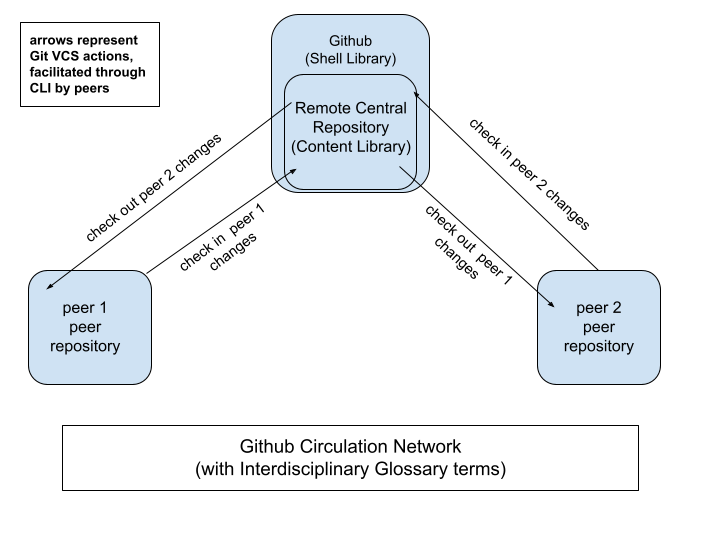
\includegraphics[width=.8\textwidth]{./images/gcn_flowchart.png}
\caption{"Illustrating the P2P GCN using interdisciplinary glossary terms."}
\vspace{0in}
\end{center}
\end{figure}

The above flowchart, similar to that in the P2P section of the Concepts chapter, approaches the same concept using the new Interdisciplinary Glossary terms. Here, the network is named Github Circulation Network, to reflect how this P2P system represents the circulation of information through Git and Github. The two lower nodes where the information originates are now labeled "peer repository", to reflect how the repositories on the local machines function as the endpoints of each peer node, and are therefore the peer's repository. The remote repository on Github has been renamed the "remote central repository" to reflect the position as the remote version of the repository on Github, and that it is the centralized piece of the P2P network. 

Additionally, note that the remote central repository includes the name "content library" and is held within another box labeled "shell library", which represents Github. The addition of this nested node structure has been added to represent how Github functions as a library entity. In physical library systems, there is often a central library and many branch libraries, which are bound to this central library in that library system. On Github however, individual repositories function as their own entities with their own development communities, held within the overall structure of Github as a "shell". Then, Github as a "shell library", includes the repositories which contain the projects and their associated communities, and therefore the content of the library. Because of this, the term "content library" has been assigned to repositories. Then, the content library sits within the shell rather than attached to, because it is part of the decentralized library-like system of Github.  

\subsection{The Community Code Archival Librarian}

The term "Community Code Archival Librarian" (CCAL) has been given to the the methodology of understanding who carries out the actions of the librarian defined by Gorman \cite{gorman2000values} and the SAA values \cite{rubin2016foundationslis} which apply to Github based on discussion in the Concepts chapter. The name "Community Code Archival Librarian" has been chosen to reflect the importance of written code and the overall work of the associated communities for FOSS projects. "Archival Librarian" has been chosen to reflect the the inclusion of both actions of the librarian and SAA values in this new term. In giving this term a name, it is necessary to note the difficulty in including the true scope of the materials this position works with archiving. For example, "code" and "community" do not accurately reflect the importance of documentation in software projects, although this is attempted to be included through the "community" aspect, as that documentation, all the issue discussion, project board organization, and pull request processes are all work of the collective FOSS community for each repository.

These are the actions of the CCAL: 
\begin{itemize}
    \item select\cite{gorman2000values}/selection\cite{rubin2016foundationslis}
    \item acquire \cite{gorman2000values}
    \item organize and give access \cite{gorman2000values}
    \item preserve and conserve \cite{gorman2000values}
    \item assist \cite{gorman2000values}
    \item instruct \cite{gorman2000values}
    \item access and use \cite{rubin2016foundationslis}
    \item accountability \cite{rubin2016foundationslis}
    \item advocacy \cite{rubin2016foundationslis}
    \item diversity \cite{rubin2016foundationslis}
    \item history and memory \cite{rubin2016foundationslis}
    \item preservation \cite{rubin2016foundationslis}
    \item professionalism \cite{rubin2016foundationslis}
    \item service \cite{rubin2016foundationslis}
    \item social responsibility \cite{rubin2016foundationslis}
    \item administer and manage 
\end{itemize}

\section{Integration of Concepts with Github}

In this section, the concepts discussed in the previous chapter will be applied to the Github repository for the pandas project to understand how this active repository and software community function as a library, and where the actions of the librarian are carried out in this specific community. Pandas has been chosen because this is a popular repository on Github with a community that seeks to fully utilize the different components of the repository structure that have been discussed in the Concepts chapter. This application of concepts to pandas will function as a case study for Github functioning as a library archive and the application of interdisciplinary glossary terms in a practical environment. 

\subsection{pandas Repository Overview}

The pandas repository is the main repository is the main repository under the pandas-dev organization on Github, According to the About section in the pandas repository, this project is a "Flexible and powerful data analysis / manipulation library for Python, providing labeled data structures similar to R data.frame objects, statistical functions, and much more"\cite{pandasrepo}. About 90 percent of the project is written in Python according to the languages bar in the Code section of the repository\cite{pandasrepo}. 

For the most rational and organized approach to discussing the application of Library Science concepts, the discussion will follow the tabs in the repository from left to right and break down the repository contents from those within that tab, beginning with the Code tab. 

\subsection{Repository Template}

The repository template refers to a blank Github repository in the state when it is first created. At this time, it includes all of the tabs mentioned, but lacks the information within and a README. This baseline repository set up to organize information by tabs and sectioned off within each page reflects Gorman's value of Rationalism by approaching the organization of information in a repository from a technical perspective which is "independent of emotions, faith, and the senses" as Gorman defines Rationalism \cite{gorman2000values}. Encapsulating information in the tab structure allows contributors to quickly switch between different parts of the repository and maintain focus on one area at a time as well. The template including the Code page with the most recent commit, repository file system, and centering the major source of documentation that is the README, which also may link the CONTRIBUTING.md file, also reflection Rubin's value of Truth and Search for Truth by making available information \cite{rubin2016foundationslis}.

\subsection{Code}

The Code tab, being the first tab to the left of all which make up the repository, essentially functions as the home page. It includes all the branches of the repository, all the commits and displays the most recent commit name and the username of the individual who pushed the commit to Github or merged the pull request, the folder structure of the repository, the README, and a sidebar which includes an about section, the license, releases, and the bar which represents the breakdown of programming languages used in the repository. 

\subsubsection{Branches}

\begin{figure}[hbt!]
\begin{center}
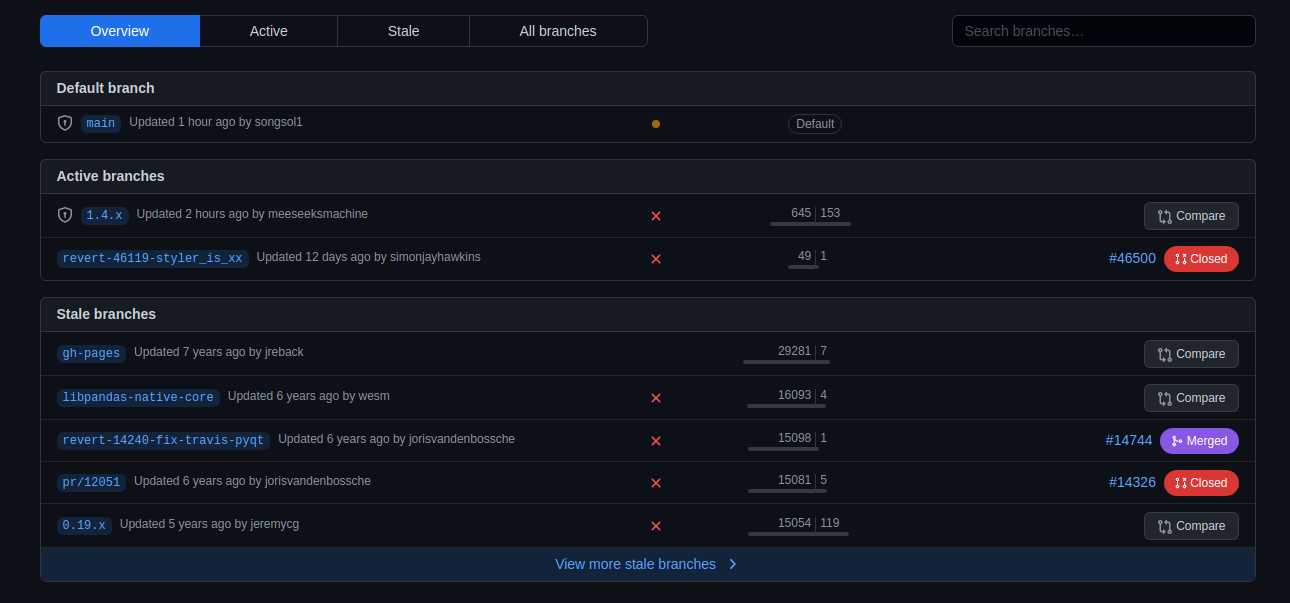
\includegraphics[width=.8\textwidth]{./images/branches.png}
\caption{"Branch page within the Code tab"}
\vspace{0in}
\end{center}
\end{figure}

Considering the use of branches is important to this research because of how the branches compare to those of a physical library system. In a physical library system, there is the central branch and other satellite branches, where information can circulate between branches, and some branches contain information which others do not. Typically, the central branch holds the largest collection. 

Branches are used as part of Git Flow to allow for collaboration of the repository without merge conflicts. A new branch is essentially another copy of only the file system in the repository. This is the file system which is brought to the local machine when "git clone" is used, and does not include the full repository structure on Github, as it lacks pieces such as the Issue Tracker and Pull Requests. This differs from a fork of a repository, which is a copy of the whole repository on Github, including all of the tabs such as the Issue Tracker and Pull Requests. 

Contributors can add new information, change existing information, and delete information in a branch and it remains local to that branch. This is then pushed to the remote branch on Github. The difference in information between a satellite branch and the main branch reflects the difference in information which occurs between branches in the circulation of information in the physical library system. In difference between the two is that the physical library allows for circulation of materials from the central branch to the satellite branch, whereas it is not possible to merge the main branch into a satellite branch on Github, it is only possible to create a pull request that merges changes from the satellite branch into the main branch. Github tracks the difference in versions in terms of commits for each branch of the repository. For example in pandas, there is a bar above the most recent commit in the 1.4.x branch which notes "This branch is x commits ahead, x commits behind main"\cite{pandasrepo}. This is an example of how Git as a version control system takes on actions of the CCAL to record the history of changes in the repository. 

\subsubsection{Commits}

The most recent commit bar includes a link at the end, which appears as a clock followed by the number of commits in the repository, excluding commits that have been squashed into one. The commits are grouped by day. The commits function as links to the diff page, which shows a side by side comparison for every file changes, with the left side showing deletions and the right side showing additions. This diff page functions as a representation of the actions that occur at the peer end of the Github Circulation Network, by showing information which has been removed from the current version of the project and therefore removed from further circulation. It is important to note that this removal is only to some extent, as it is not possible to remove this from previously existing forks that have not been merged or commit-absent copies. Commit "Fix CI" in the pandas repository will be considered as an example for understanding the Github Circulation Network in a practical application. 

\begin{figure}[hbt!]
\begin{center}
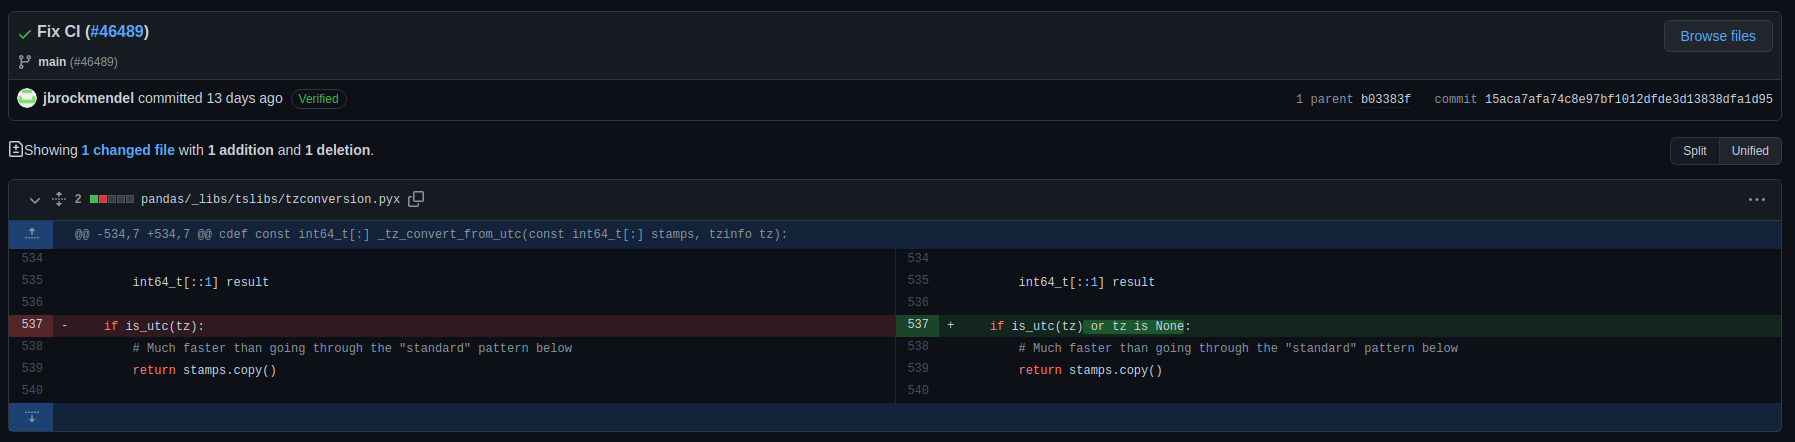
\includegraphics[width=.8\textwidth]{./images/fix_CI_diff.png}
\caption{"Fix CI commit diff page to view changes made"}
\vspace{0in}
\end{center}
\end{figure}

Commit "Fix CI" , pushed to Github by jbrockmendel, includes a change in an if statement they made on line 537 of the file tzconversion.pyx, as shown on the diff page for this commit, which adds to the end of the existing if statement "or .tz is None" \cite{pandasrepo}. As a result of this change in the main branch of the repository, local versions of the repository which have not checked out this new version have now become commit-absent copies of the repository because they are behind in the commit history. As previously stated, this diff page represents the change which was made in the peer repository of the Github Circulation Network. Then, this addition went through the add/commit/push process using Git, which shared this information to the remote central repository on Github. Now that the change in this if statement is in the remote central repository, other peers in this network are able to check out the new version of the repository to their peer repository, completing the full peer-to-peer process of the Github Circulation Network. 

\subsubsection{Releases and Packages}

Similar to commits, releases and packages are a way in which Github functions as a version control system. According to the Packages section of the pandas repository, there are no packages available, so this section will instead focus on releases since this is utilized by pandas \cite{pandasrepo}. Each new release functions as an update for the pandas tool, facilitated through the Git command "tag" by maintainers of the repository \cite{gitdocs}. On the Release page, it is possible to choose between seeing full releases or the list of tags, which are the version of the releases. Each release on the Release page still includes the tag number. For example, the most recent release was facilitated by simonjayhawkins and the tag for the release was 1.4.1 \cite{pandasrepo}. The preservation of the code and documentation in this release reflects Rubin's value of The Public Good, characterized by Rubin as "preserving the cultural record" \cite{rubin2016foundationslis}. This is because each release includes the source code at the time of that release, which is preserved in that state even when future releases are made. The source code qualifies as cultural record because it is a result of the collaboration of the pandas community, and includes the contributions of many people. There may be contributions which are altered in future releases, but remain intact from how the original author created them in the 1.4.1 release. 

Additionally, multiple actions of the CCAL have been carried out for releases. As a maintainer making releases, simonjayhawkins has carried out the action of Select by choosing the point at which the release would be made and no further changes would be included in the 1.4.1 release \cite{gorman2000values}\cite{rubin2016foundationslis}. The action of Organize and Give Access was taken, because there are CLI commands given along with the release to download and upgrade pandas to the new version \cite{gorman2000values}. These commands may also fall under Instruct since the commands could be considered instruction for download \cite{gorman2000values}. Lastly, the record of the release would qualify as an act of preservation for preserving the project code in the moment of the release without accounting for future changes made after the release date, which is Feburay 12th, 2020 for 1.4.1 \cite{rubin2016foundationslis}\cite{pandasrepo}.

\begin{figure}[hbt!]
\begin{center}
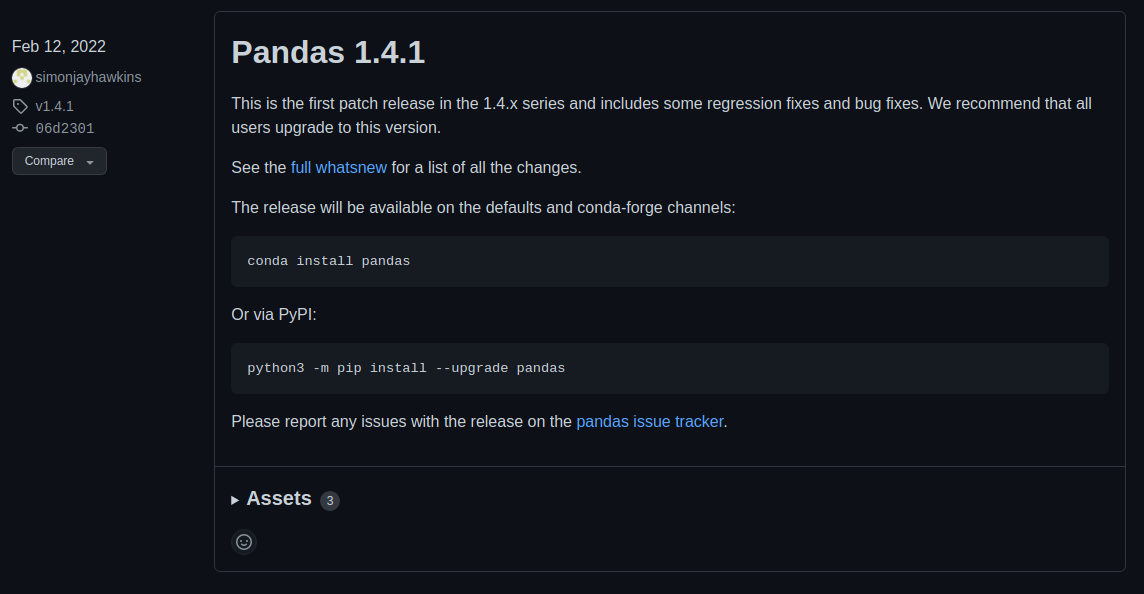
\includegraphics[width=.8\textwidth]{./images/releases.png}
\caption{"Release 1.4.1"}
\vspace{0in}
\end{center}
\end{figure}

\subsubsection{README}

An interesting quality of the README is that it is not immediately part of the repository template. Rather, the template prompts the repository owner to create a README, and READMEs are considered to be best practice for using Github. The README being a markdown file includes crucial information about the project and contributing to it. The README itself through the organization of information using headers and lists available in Markdown reflects Gorman's value of Rationalism \cite{gorman2000values}. In the pandas repository, the README includes several sections: buttons with key information (such as version number, license, and code testing coverage), What is it, Main Features, Where to get it, Dependencies, Installation from sources, License, Documentation, Background, Getting Help, Discussion and Development, and Contributing to pandas\cite{pandasrepo}. 


The README being the major source of documentation in the repository also reflects Gorman's value of Literacy and Learning \cite{gorman2000values}. This is a less specific application because the users and contributors must seek out the information in the README, although they can certainly ask questions to the project's community through the issue tracker. The README also takes on Gorman's Librarian action of Assist Library Users \cite{gorman2000values}, which also falls under the actions of the CCAL as defined in the Interdisciplinary Glossary. In this case, it could be considered either Github or the contributors who ultimately carry out this action because Github holds the README file but this is not included in the repository template, and must be organized and filled with information by the contributors and maintainers. In pandas, the Assist would be reflected through the contributing guidelines in the pandas documentation, which is linked in the README file but hosted on a separate website specifically for documentation. The inclusion of documentation for contributing reflects the CCAL action of preservation \cite{rubin2016foundationslis}. 

\subsection{Issues}

The Issue Tracker can be sorted between both open and closed issues, keeping record of all prior issues and the comments within even once the issue is closed. It is possible to filter through the issues by author, label, projects, milestones, and the assignee. There are labels given by the repository template, but it is possible to add new labels or more specific organization. Pandas had utilized this feature, adding labels such as Admin for "administrative tasks", CI for "continuous integration", and Linux for "Linux OS" within the total of 130 different labels \cite{pandasrepo}. The use of many labels to organize the issues might be considered classification, which Gorman includes in defining the action of Organize and Give Access \cite{gorman2000values}. The labels also help the contributors and maintainers better access specific information by searching for labels. By applying the labels to issues contributors and maintainers are carrying out actions of the CCAL, as Organize and Give Access is considered one of those actions.

\subsubsection{Open Issues}

Issue 46485 BUG: isin() give incorrect results for uint64 columns will be considered as an example of an open issue, because it includes discussion through comments between two contributors \cite{pandasrepo}. The issue was opened by AlexSingle, who carried out the actions of a CCAL as discussed above by adding the labels "Bug" and "Needs Triage" to the issue after it was created \cite{pandasrepo}. Contributor Saxeman commented on the issue to claim it, and was automatically assigned to the issue by the github-actions bot \cite{pandasrepo}. The github-actions bot in this instance acts as the CCAL through the action of Organize and Give Access by "maintaining online systems" \cite{gorman2000values}. 

\begin{figure}[hbt!]
\begin{center}
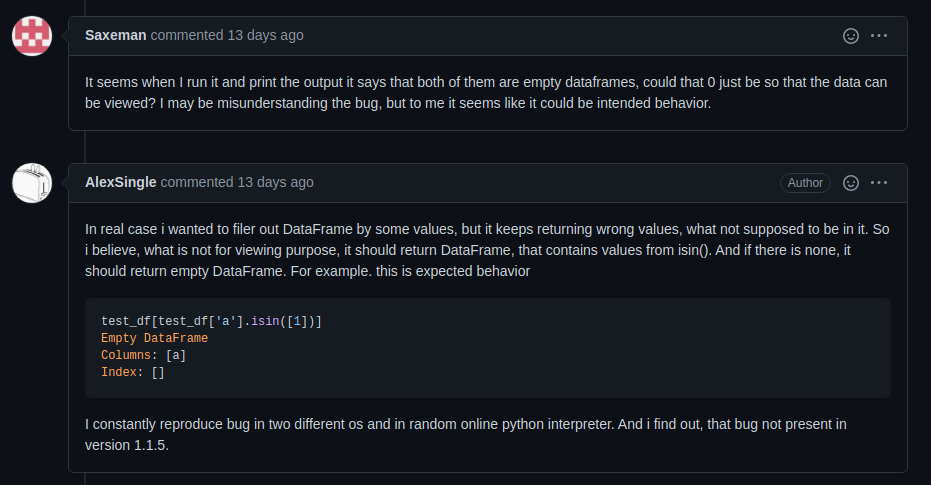
\includegraphics[width=.8\textwidth]{./images/issue_discussion.png}
\caption{"Discussion in Issue Tracker on Issue 46485"}
\vspace{0in}
\end{center}
\end{figure}

Over a few comments on this issue, Saxeman asks a question to AlexSingle to better understand the bug and another follow up question, which AlexSingle answers with code examples \cite{pandasrepo}. The documentation of this conversation in the issue tracker reflects Github carrying out the actions of the CCAL through Accountability, by keeping record of the conversation which will remain recorded even once the issue is closed \cite{rubin2016foundationslis}. Additionally, Tolerance is present here through the discussion between the two contributors with the goal of understanding how the bug worked in order to find a solution \cite{rubin2016foundationslis}. In this instance AlexSingle responding with guidance for understanding the bug is an instance of the Assist action \cite{gorman2000values}. 

\begin{figure}[hbt!]
\begin{center}
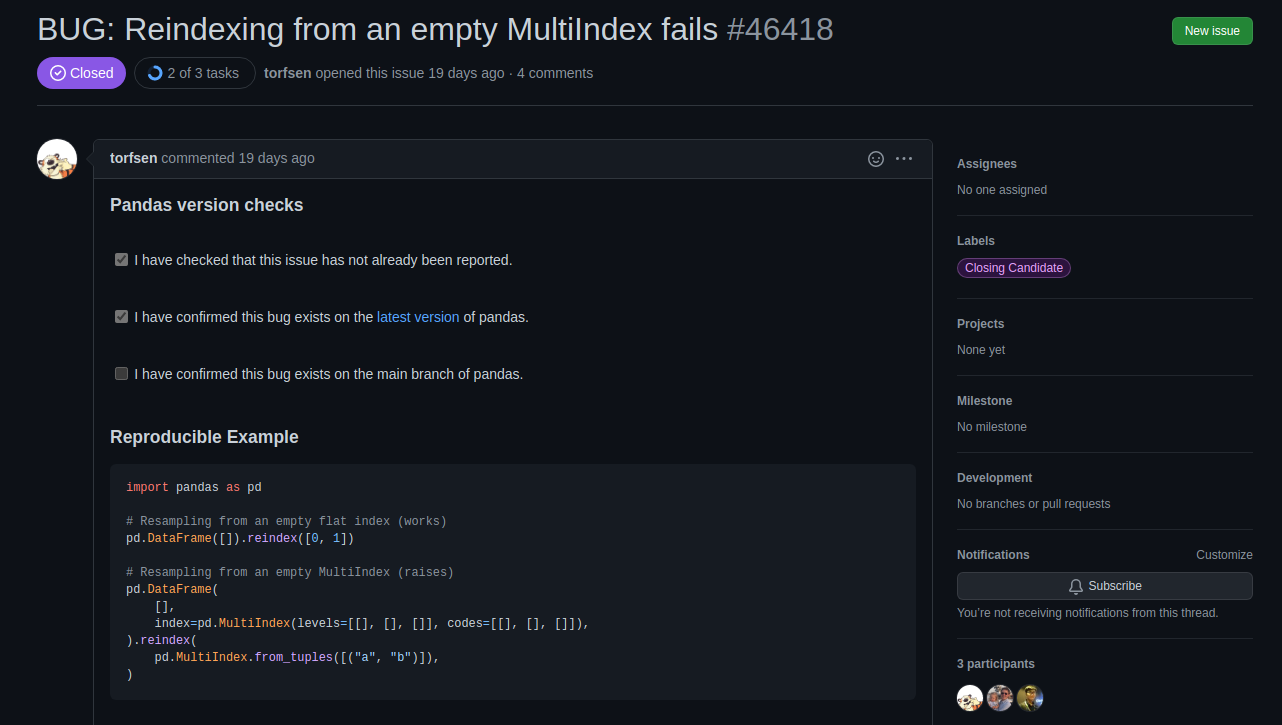
\includegraphics[width=.8\textwidth]{./images/closed_issue.png}
\caption{"Closed Issue 46418"}
\vspace{0in}
\end{center}
\end{figure}

\subsubsection{Closed Issues}

An an example of a Closed Issue, Issue 46418 will be considered, which is titled BUG: Reindexing from an empty MultiIndex fails \cite{pandasrepo}. By Github keeping record of all issues once they are closed, the platform is taking on qualities of the library and actions of the CCAL. First, Github is engaging in the core value of Stewardship by keeping record of the full conversation, which may be considered "preserving the human record" since this conversation is record of the open source community interactions \cite{gorman2000values}. Additionally Archivist values of history and memory, as well as preservation are present as the closed issue remains preserved by Github and it becomes part of the history of the community associated with the pandas repository \cite{rubin2016foundationslis}.

\subsection{Pull Requests}

The main page of the Pull Request tab appears in exactly the same format as the Issues tab, including the pages of open and closed issues, the drop down tabs to sort by author and so on, and the same 130 labels available to organize issues \cite{pandasrepo}. Open PRs have not been merged or closed and are indicated by the green icon. Closed PRs are usually merged, indicated by the purple icon, but may remain unmerged, indicated by the red icon. Because of the similarity between the Issues and Pull Request as community discussion spaces local to Github and their overall format, both will share actions of the CCAL and qualities of libraries that apply. 

In an open source project like pandas where commits must be merged into the project in order for the commits to be part of the main branch and new releases (unless further changes are made to that work), pull requests function as the last step of the Github Circulation Network. Although the contributions of all contributors remain recorded in branches in the repository and forks on Github, this likely is not being used by other contributors and users like the main pandas project would be. 

The major difference between pull requests and issues is that pull requests function as part of the Github Circulation Network, while issues do not. The pull request, as mentioned, is the final step in the Github Circulation Network for checking in new information in FOSS projects because it is the addition of the commits into the main branch of the repository, where those changes can be pulled to peer repositories, completing the network. There may also be a difference in how Selection occurs at the PR stage, as this occurs after development has occurred, where discussion in the Issue Tracker occurs before or during development \cite{gorman2000values}\cite{rubin2016foundationslis}. 

\subsubsection{Open Pull Request}

\begin{figure}[hbt!]
\begin{center}
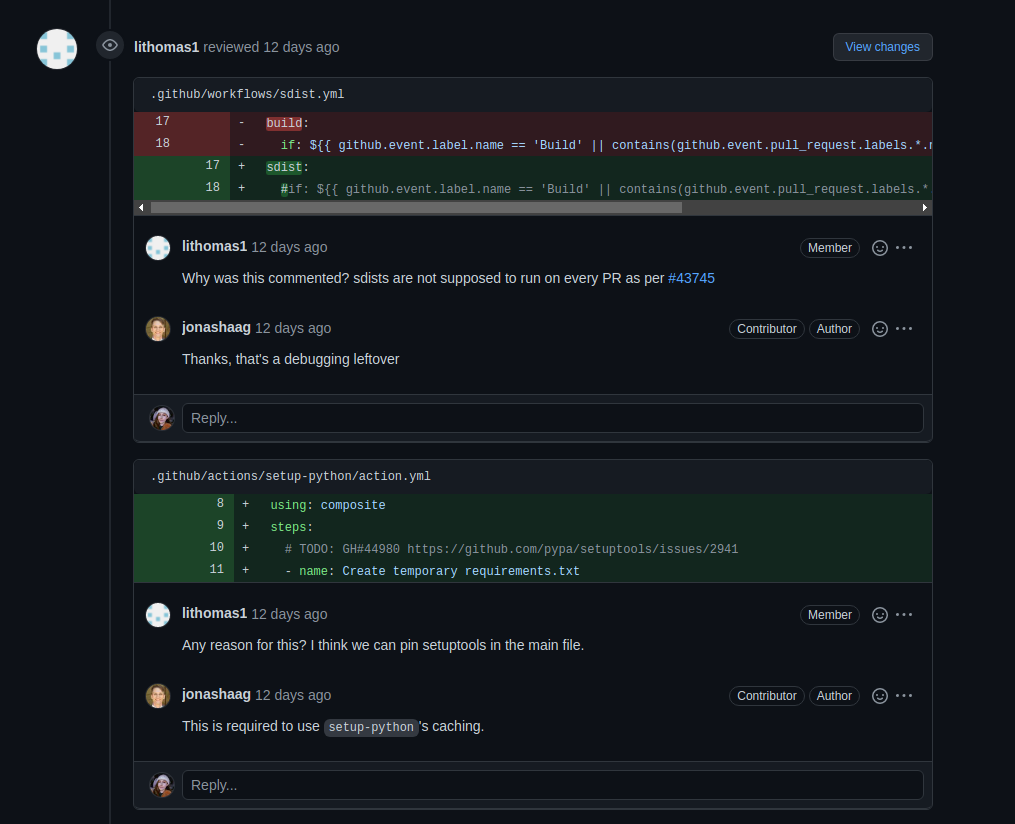
\includegraphics[width=.8\textwidth]{./images/pr_review.png}
\caption{"PR Review by maintainer on PR 46493 Refactor CI"}
\vspace{0in}
\end{center}
\end{figure}

Pull Request 46493 Refactor CI will be considered as an example of an open pull request due to the documentation of a conversation on what changes should be included in the final merge \cite{pandasrepo}. Through the discussion in the comments of the PR, the contributors are deciding what will and will not be included in the potential merge. By submitting a pull request, contributor jonashaag is engaging in Gorman's value of Intellectual Freedom to some extent, by showing their commits which they wish to be part of the project \cite{gorman2000values}. However, whether these commits are merged into the project is ultimately the choice of the maintainers, and changes may be requested to the existing work before it is merged. Reviewer lithomas1, acting as the maintainer by reviewing jonashaag's PR, added two comments with changes/questions. By reviewing this PR, lithomas1 is acting in service for the development community of pandas, which is an example of Rubin's value of Service, "underlying the value of service is the belief in the betterment of the individual and the community as a whole" \cite{rubin2016foundationslis}. This action of reviewing the pull request also qualifies as an action of the CCAL through the archivist action of service \cite{rubin2016foundationslis}. Because the conversation through open pull requests determined what is and is not merged into the project, jonashaag and lithomas1 are both carrying out the actions of the CCAL, specifically Gorman's library action of Select and the archivist action of selection \cite{rubin2016foundationslis} \cite{gorman2000values}. After lithomas1's review, other maintainers join the conversation of the pull request

\subsubsection{Closed Pull Requests}

Similar to how Github handles closed issues, the full record of the pull request including comments is preserved on Github under the closed PR section of the Pull Request tab. For PRs, the state of the pull request at the time of closing it is also recorded, whether it was merged or closed. Closed PRs, both merged and closed without merging, will be studied. 

For the PR closed without merging, PR 46531 change default value (for index) of func named to\_cvs created by a5chin will be studied \cite{pandasrepo}. In the comments of this issue, maintainer jreback is the reviewer of the PR and engages in discussion about there not being an issue associated with the pull request, which is required for the change a5chin would like to merge into the project \cite{pandasrepo}. Another maintainer, mroeschke, comments on the PR confirming that there needs to be community discussion through an issue, and notes that they will close the PR until that discussion occurs \cite{pandasrepo}. In this instance, the maintainers are upholding the CCAL value of Professionalism by requiring the contributor to follow the issue tracker discussion step of the contributing process \cite{rubin2016foundationslis}. Similar to how Github preserves the conversation with issues, the value of Stewardship applies to how Gitub keeps record of the umerged PR, which shows the value of recording the community interaction and all contribution, even if that contribution is incomplete and not included in the project \cite{gorman2000values}. However, in the case of PR 46531, Github's ability to carry out Stewardship to the full extent of documenting the commits as part of this PR is complicated by a5chin's choice to completely delete the branch holding their work \cite{pandasrepo}. This could negatively impact the community by deleting work which could have been merged if an issue had been created for community discussion, as requested by the maintainers. Even if the work was abandoned by a5chin, maintainers or other contributors could have picked up the work and continued with it. Because Github has preserved this closed PR, it may still be possible to salvage the available information about the work from the comments. Evidently, Github has acted as the CCAL here through the values of history and memory, and preservation \cite{rubin2016foundationslis}. It is possible to see through the record of conversation and the last action notes on the PR of a5chin deleting the branch how recorded code can be lost, and understand the potential consequences for the community when a contributor withdraws their work, which qualifies this as valuing history and memory \cite{rubin2016foundationslis}.

\begin{figure}[hbt!]
\begin{center}
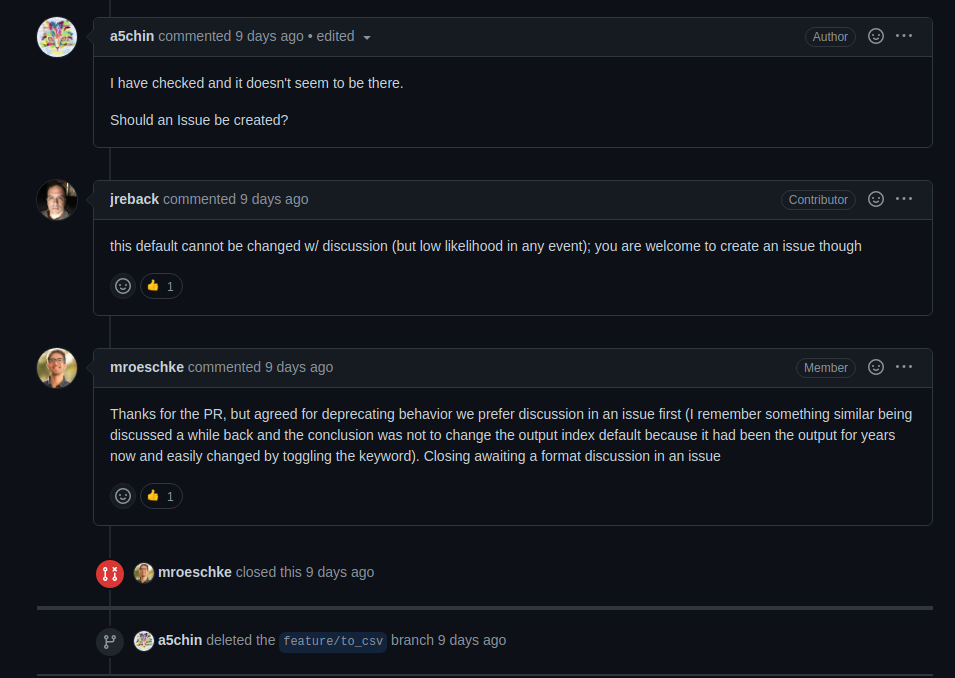
\includegraphics[width=.8\textwidth]{./images/closed_no_merge.png}
\caption{"PR closed without merging"}
\vspace{0in}
\end{center}
\end{figure}

\begin{figure}[hbt!]
\begin{center}
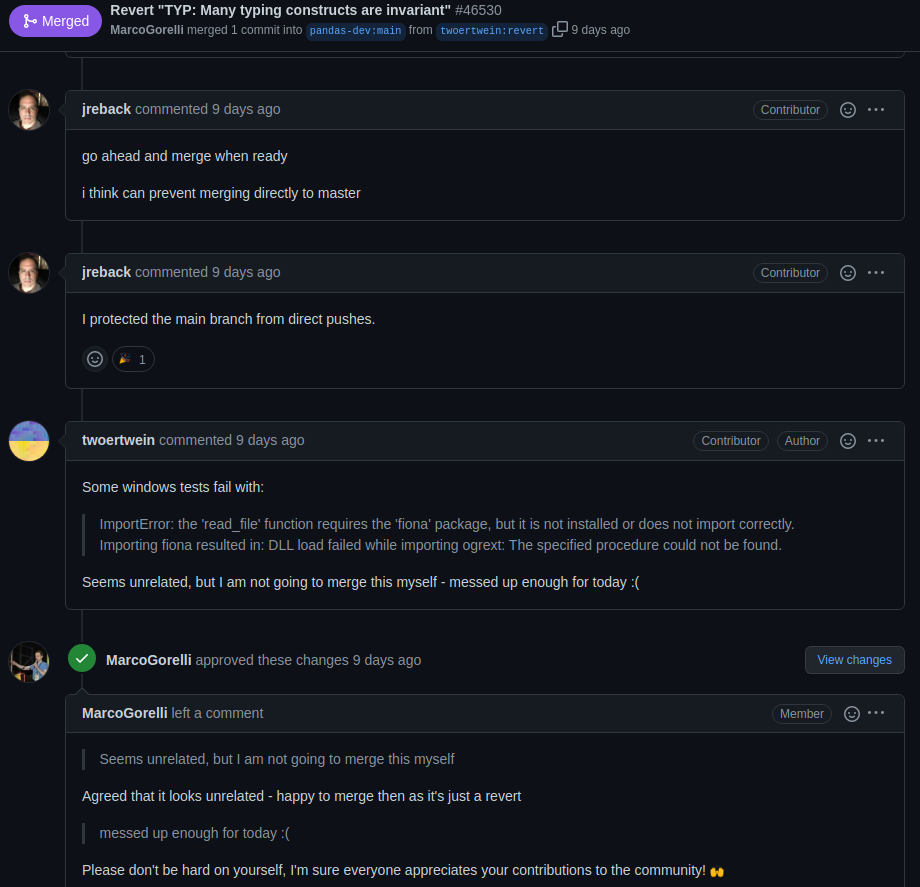
\includegraphics[width=.8\textwidth]{./images/merged_pr.png}
\caption{"Discussion between contributor and maintainers on PR closed due to merge"}
\vspace{0in}
\end{center}
\end{figure}

For the pull request which has been closed due to a merge, PR 46530 Revert "TYP: Many typing constructs are invariant" will be studied \cite{pandasrepo}. According to the PR title and comments from twoertwein, the contributor who opened the PR, this PR reverts to a prior version of pandas because twoertwein pushed to the main branch rather than their own \cite{pandasrepo}. Two maintainers, jreback and MarcoGorelli, review the changes and stop other commits from being able to be pushed to main \cite{pandasrepo}. MarcoGorelli specifically addresses twoertwein's concerns about completing the merge for this PR successfully, comments with reassurace about their work being valued for the project, then completes the merge for the PR \cite{pandasrepo}. In this PR, MarcoGorelli and jreback are upholding the value of service for the pandas community by reviewing this PR, and MarcoGorelli by giving encouragement to a member of the community and therefore helping create a positive community space even when a contributor makes the mistake of pushing to the wrong branch \cite{pandasrepo}\cite{gorman2000values}\cite{rubin2016foundationslis}. In this instance, jreback as a maintainer carries out the CCAL action of organize and give access by restricting push access to the main branch of the pandas repository \cite{gorman2000values}. The same actions of the CCAL which applied to the closed unmerged pull request apply to this PR, with the additional understanding that Github carries out the actions of Social Responsibility and Accountability through preserving the comments of the pull request, which are just one piece of the interactions in the pandas community and can be used to verify the actions of community members \cite{rubin2016foundationslis}. By revoking the ability to push directly to the main branch, maintainers jreback and MarcoGorelli are carrying out the CCAL action of access and use \cite{rubin2016foundationslis}, in addition to administer and manage\cite{gorman2000values}. 

\subsection{Actions}

In a Github repository, the Actions tab shows a list of all the bots which operate within that repository. When the name of the bot in clicked on, it shows a link to the .yml file which controls the actions of the bot and the list of contributors who built it. Underneath this link is a list of all the instances where the bot was run, which are called workflows, including the total number of workflows for the full history of the bot. These records of each workflow run include the contributor whose action caused the bot to run a workflow, what the status of the workflow is, and the time it lasted \cite{pandasrepo}.

\subsubsection{Bots in Maintaining Repositories}

\begin{figure}[hbt!]
\begin{center}
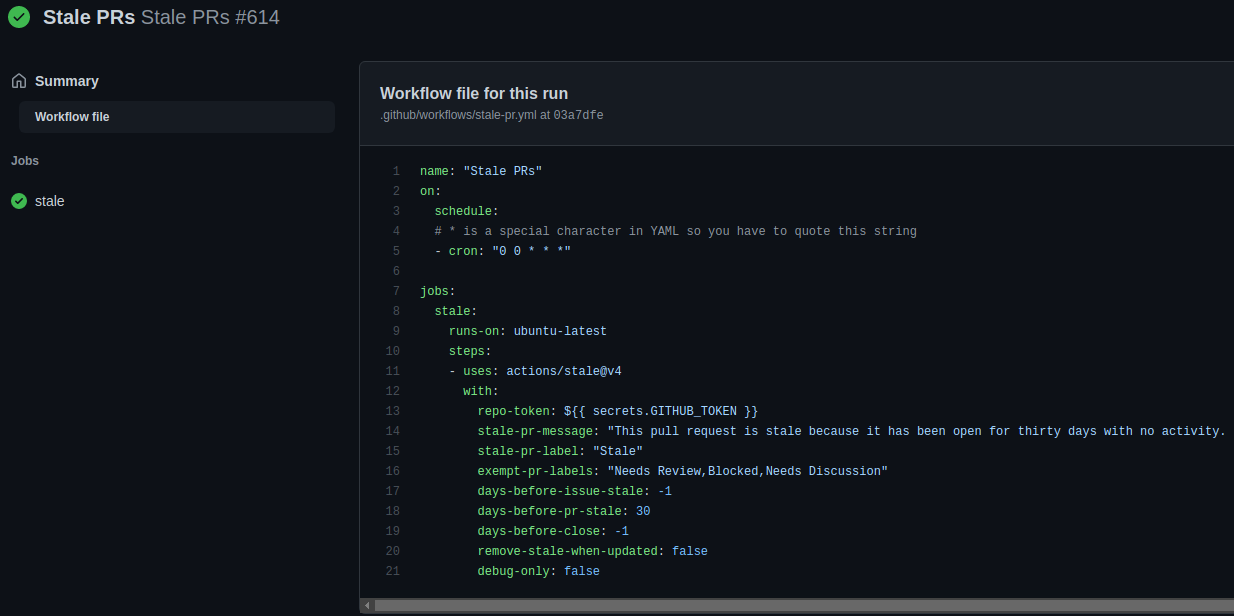
\includegraphics[width=.8\textwidth]{./images/actions_pr_bot.png}
\caption{"Code file for the Stale PR bot."}
\vspace{0in}
\end{center}
\end{figure}

Considering the Stale PRs bot, the last workflow was run according to the schedule it is based on and this workflow run was a success, and this workflow lasted 53 minutes \cite{pandasrepo}. Looking at stale-pr.yml, it is shown that two maintainers built this file rather than the bot being part of Github, which qualifies as the maintainers carrying out the CCAL action of service by creating a bot that serves the community \cite{gorman2000values} \cite{rubin2016foundationslis}. Because the service to the project community in maintaining stale PRs is carried out by the bot, the action of service applies to the Stale PRs bot as well \cite{gorman2000values} \cite{rubin2016foundationslis}. In building the bot, the maintainers are ensuring that the CCAL actions organize and give access, preserve and conserve, and preservation are carried out in the Pull Requests by the bot. Organize and give access applies because the PRs are closed after 30 days of no activity and recorded so that they may be opened again in the future, which preserves them but helps keep the open PRs limited to active conversation and activity \cite{gorman2000values} \cite{rubin2016foundationslis} \cite{pandasrepo}. Lastly, the value of Stewardship applies to the bot's actions of closing the PR and to Github's practice of recording closed PRs because the PRs are preserved in the closed state rather than being deleted \cite{gorman2000values}. 

\subsection{Projects}

\begin{figure}[hbt!]
\begin{center}
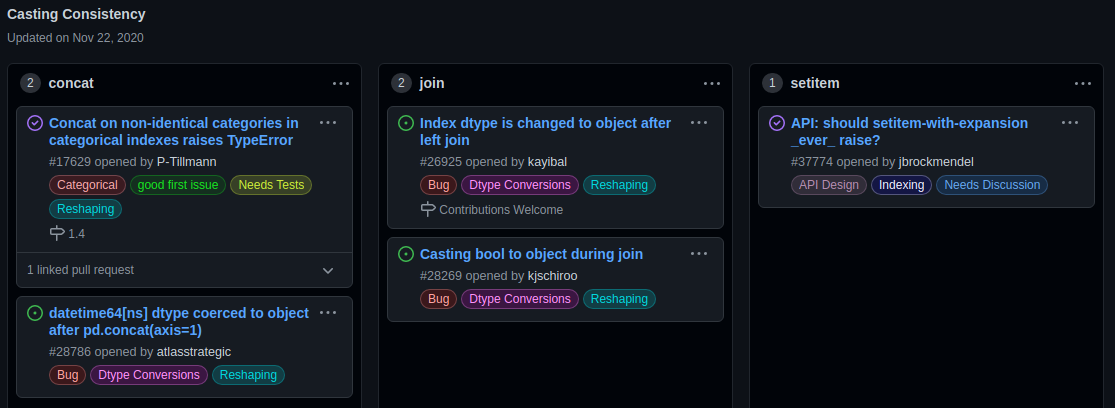
\includegraphics[width=.8\textwidth]{./images/project_board.png}
\caption{"Active project board in pandas."}
\vspace{0in}
\end{center}
\end{figure}

The Projects tab in the repository template is initially blank, allowing for maintainers and the community to sort issues into categories to better track the completion of a project and understand what needs to be done in what area of the project \cite{pandasrepo}. This is a space that can be used by both maintainers and contributors, as it is available to the whole community in pandas. The in-progress project Casting Consistency will be studied as an example of a project in pandas \cite{pandasrepo}. There are three columns, labeled from left to right as concat, join, then setitem \cite{pandasrepo}. Each include issues as the content of the columns, which shows the name of the issue and the tags given to the issue, which is show in a sidebar view when the title is clicked \cite{pandasrepo}. The overall structure given by Github to categorize issues reflects Gorman's value of Rationalism, shown here through the discrete, technical organization that the contributors and maintainers of pandas have chosen to use for the Casting Consistency project \cite{gorman2000values} \cite{pandasrepo}. The content of issue within the category directly applies to the title of the category. For example, the first of the two issues in the concat column is titled "Concat on non-indentical categories in categorical indexes raises TypeError" \cite{pandasrepo}. Because the projects tab is more about organization for the project community than recording information, the application of Library Science concepts is limited to Rationalism in the Projects tab. 

\subsection{Wiki}

The Wiki tab functions as a collection of links to different resources and documentation for the pandas community \cite{pandasrepo}. The main page of the Wiki includes a main section with headers: External Links (includes Docs and API reference), Reference, For Documentation Authors, For Developers (noted as being moved soon, with a link to "complete documentation"), and For Maintainers \cite{pandasrepo}. There is also a sidebar with more information for maintainers and developers, under a drop down menu of all 29 pages of the Wiki \cite{pandasrepo}. The Wiki for pandas as a whole being a rich source of documentation for understanding and contributing to the project and on Github in general qualifies the Wiki as an example of Literacy and Learning \cite{gorman2000values}. There is the complication here of the user or the contributor needing to actively seek out this information, but this process is made easier by the Wiki holding this information, and being organized into pages, including a main page with sections of information \cite{pandasrepo}. The Truth and Search for truth applies in this instance as well, because of how the Wiki more easily makes available information to those who are seeking it \cite{rubin2016foundationslis}. The Wiki also functions as the CCAL through holding information that assists and instructs both users and contributors, and professionalism through providing access to the information that guides the actions of contributors and maintainers, such as the contributing guidelines \cite{gorman2000values} \cite{rubin2016foundationslis} \cite{pandasrepo}. More specifically, the information in the pandas Wiki which by being included qualifies this as assist and instruct Using Git under the For Developers header, or the link to Google Summer of Code being included \cite{pandasrepo} \cite{rubin2016foundationslis}. For Maintainers, this would include guidelines for the merge and release processes \cite{pandasrepo}. By including access to this information, especially Google Summer of Code, pandas may be indirectly advocating for Coding Literacy by surfacing this resource \cite{vee2017coding}. 

\subsection{Security}

The Security tab includes both the Security Policy and any Security advisories associated with the repository, and although there are no security advisories on pandas, there is an active security policy\cite{pandasrepo}. When the security policy link is clicked, it redirects to a .gtihub.SECURITY.md file which links to the Tidelift website for reporting a vulnerability \cite{pandasrepo}. By including the ability for users, contributors, and maintainers to report vulnerabilities through Tidelift , the value of Privacy applies to the pandas repository \cite{gorman2000values}. According to the Tidelift security policy, "Tidelift acts as the security contact for many open source projects" \cite{tideliftpolicy}.

Taking a closer look at the Tidelift page for their security policy, this application takes an extra step in security for the reporter by providing a public key to encrypt the email when reporting vulnerabilities to Tidelift \cite{tideliftpolicy}. By providing the public key, this security service is giving an extra level of privacy for the reporter, again reflecting the value of Privacy \cite{gorman2000values}. 

\subsection{Insights}

\begin{figure}[hbt!]
\begin{center}
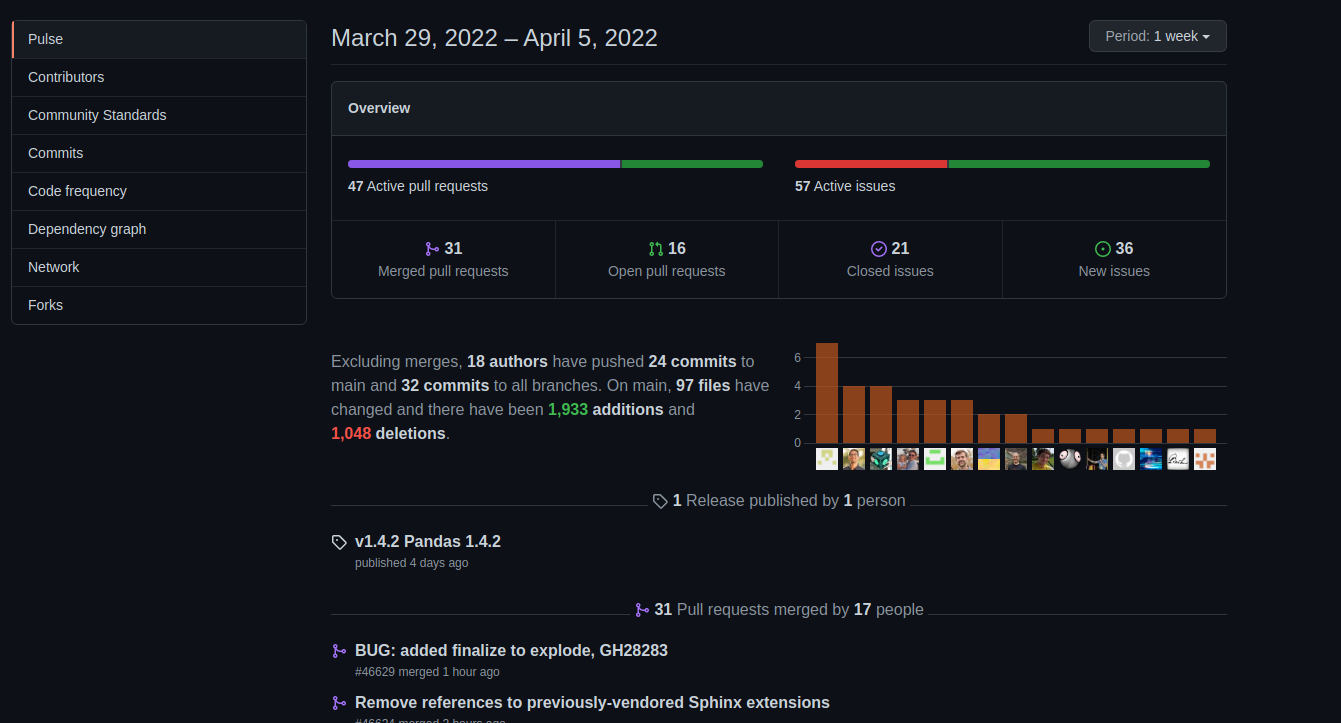
\includegraphics[width=.8\textwidth]{./images/insights.png}
\caption{"Main page of the Insights tab in pandas."}
\vspace{0in}
\end{center}
\end{figure}

Insights is the final tab in a Github repository, which includes extensive data about the repository and the community \cite{pandasrepo}. This tab is organized by Github itself, rather than being worked on by maintainers or contributors, therefore the values and actions which apply to the Insights tab apply to Github directly.  The first page, labeled "Pulse" shows graphs and lists of repository activity over a certain period of time, such as a week \cite{pandasrepo}. Through recording all contributions from all contributors in the issues and PRs, Github is engaging in the CCAL value of diversity,\cite{rubin2016foundationslis}. Additionally, values which are strongly present in the insights is preserve and conserve, as well as history and memory, because the insights tab specifically is a record of the history of the whole pandas development community \cite{rubin2016foundationslis} \cite{pandasrepo}. Graphs of commit activity for commits in the main branch are shown for each contributor, and for the repository as a whole \cite{pandasrepo}. An interesting piece of the Insights tab is the Community Standards page, which evaluates on a checklist and shown with an orange/yellow/green gradient bar the way in which the project meets best practices considered by Github \cite{pandasrepo}. This includes checks for a README, Contributing guidelines, and a License, with the only missing check being "Repository admins accept content reports" \cite{pandasrepo}. By Github including this checklist, Github is carrying out the CCAL action of accountability \cite{rubin2016foundationslis}. 

\subsection{Case Study Concluding Overview}

To summarize, this case study to analyze how Github functions as a library archive has been implemented with pandas because this a repository with high activity and an extensive community of maintainers and contributors who use Github and Git extensively, including a full range of the functions allowed by the repository. In the pandas repository, the following values of libraries and library and information science applied: 

\begin{itemize}
  \item Rationalism \cite{gorman2000values}
  \item Literacy and Learning \cite{gorman2000values}
  \item The Public Good \cite{rubin2016foundationslis}
  \item Tolerance \cite{rubin2016foundationslis}
  \item Stewardship \cite{gorman2000values}
  \item Intellectual Freedom \cite{gorman2000values}
  \item Service \cite{gorman2000values} \cite{rubin2016foundationslis}
  \item Truth and Search for Truth \cite{rubin2016foundationslis}
  \item Privacy \cite{gorman2000values}
\end{itemize}


The following CCAL actions applied to Github and the community: 

\begin{itemize}
  \item Select \cite{gorman2000values} \cite{rubin2016foundationslis}
  \item Organize and Give Access \cite{gorman2000values}
  \item Access and Use \cite{rubin2016foundationslis}
  \item Instruct \cite{gorman2000values}
  \item Assist \cite{gorman2000values}
  \item Preservation/Preserve and Conserve  \cite{rubin2016foundationslis} \cite{gorman2000values}
  \item Accountability \cite{rubin2016foundationslis}
  \item History and Memory \cite{rubin2016foundationslis}
  \item Service \cite{rubin2016foundationslis}
  \item Select/Selection \cite{gorman2000values} \cite{rubin2016foundationslis}
  \item Professionalism \cite{rubin2016foundationslis}
  \item Social Responsibility \cite{rubin2016foundationslis}
  \item Diversity \cite{rubin2016foundationslis}
  \item Administer and Manage \cite{gorman2000values}
\end{itemize}


As mentioned in the Wiki, advocating for coding literacy is loosely present through the inclusion of resources for learning to code there, such as Google Summer of Code. Lastly, the centralized peer-to-peer Github Circulation Network is evident in the pandas repository through the use of the full add/commit/push process with the additional pull request step since pandas is open source, and the frequent merging of pull requests into main \cite{pandasrepo}. 



